\documentclass{article}%
\usepackage[T1]{fontenc}%
\usepackage[utf8]{inputenc}%
\usepackage{lmodern}%
\usepackage{textcomp}%
\usepackage{lastpage}%
\usepackage{amsmath}%
\usepackage{amssymb}%
\usepackage{nccmath}%
\usepackage{hyperref}%
\usepackage{float}%
\usepackage[encoding,filenameencoding=utf8]{grffile}%
\usepackage{graphicx}%
%
\hypersetup{
    colorlinks=true,
    linkcolor=blue,
    filecolor=magenta,      
    urlcolor=cyan,
    }%
\title{Implementation of machine learning for the optimization of molecular systems in solar cells}%
\author{Andrés D. Suarez{-}Guarnizo}%
\date{\today}%
%
\begin{document}%
\normalsize%
\maketitle%
\section{Abstract}%
\label{sec:Abstract}%
Las células solares orgánicas nos muestran un camino interesante hacia el uso de energías renovables ecológicas y amigables. Eso nos ayudará a mitigar el efecto o huella de carbono. Se están cuestionando formas eficientes de convertir la energía solar en electricidad, como el uso de materiales, buscando las mejores propiedades que permitan una óptima conversión energética. Este trabajo explora el uso de técnicas de aprendizaje automático (ML) para ayudar a optimizar propiedades moleculares como el orbital molecular de alta ocupación (HOMO) y las energías de orbital molecular desocupado más bajo (LUMO), así como el cálculo y calibración de la eficiencia de conversión de potencia (PCE). ) con el ánimo de buscar grandes candidatas a moléculas orgánicas para su uso como sistemas donante{-}receptor en células solares. En particular, probamos una calibración del proceso gaussiano como un modelo ML en un conjunto de moléculas reportadas en la literatura {[}1{]} y discutimos algunos aspectos tanto de las propiedades químicas como de la ventaja de usar ML%
Keywords: Organic Solar Cell, Small Molecules, Machine Learning, Computational Chemistry, Quantum Systems.

%
\section{Avances recientes}%
\label{sec:Avancesrecientes}%
ORCA es un programa flexible para química computacional que hace especial énfasis en propiedades espectroscópicas de moléculas de capa abierta. Trata una gran variedad de métodos de química cuántica desde métodos semiempíricos, la teoría del funcional de la densidad (Density Functional Theory, DFT), hasta métodos~ab initio~simples y de multireferencia, así como efectos relativísticos y medioambientales.%


\begin{figure}[h!]%
\centering%
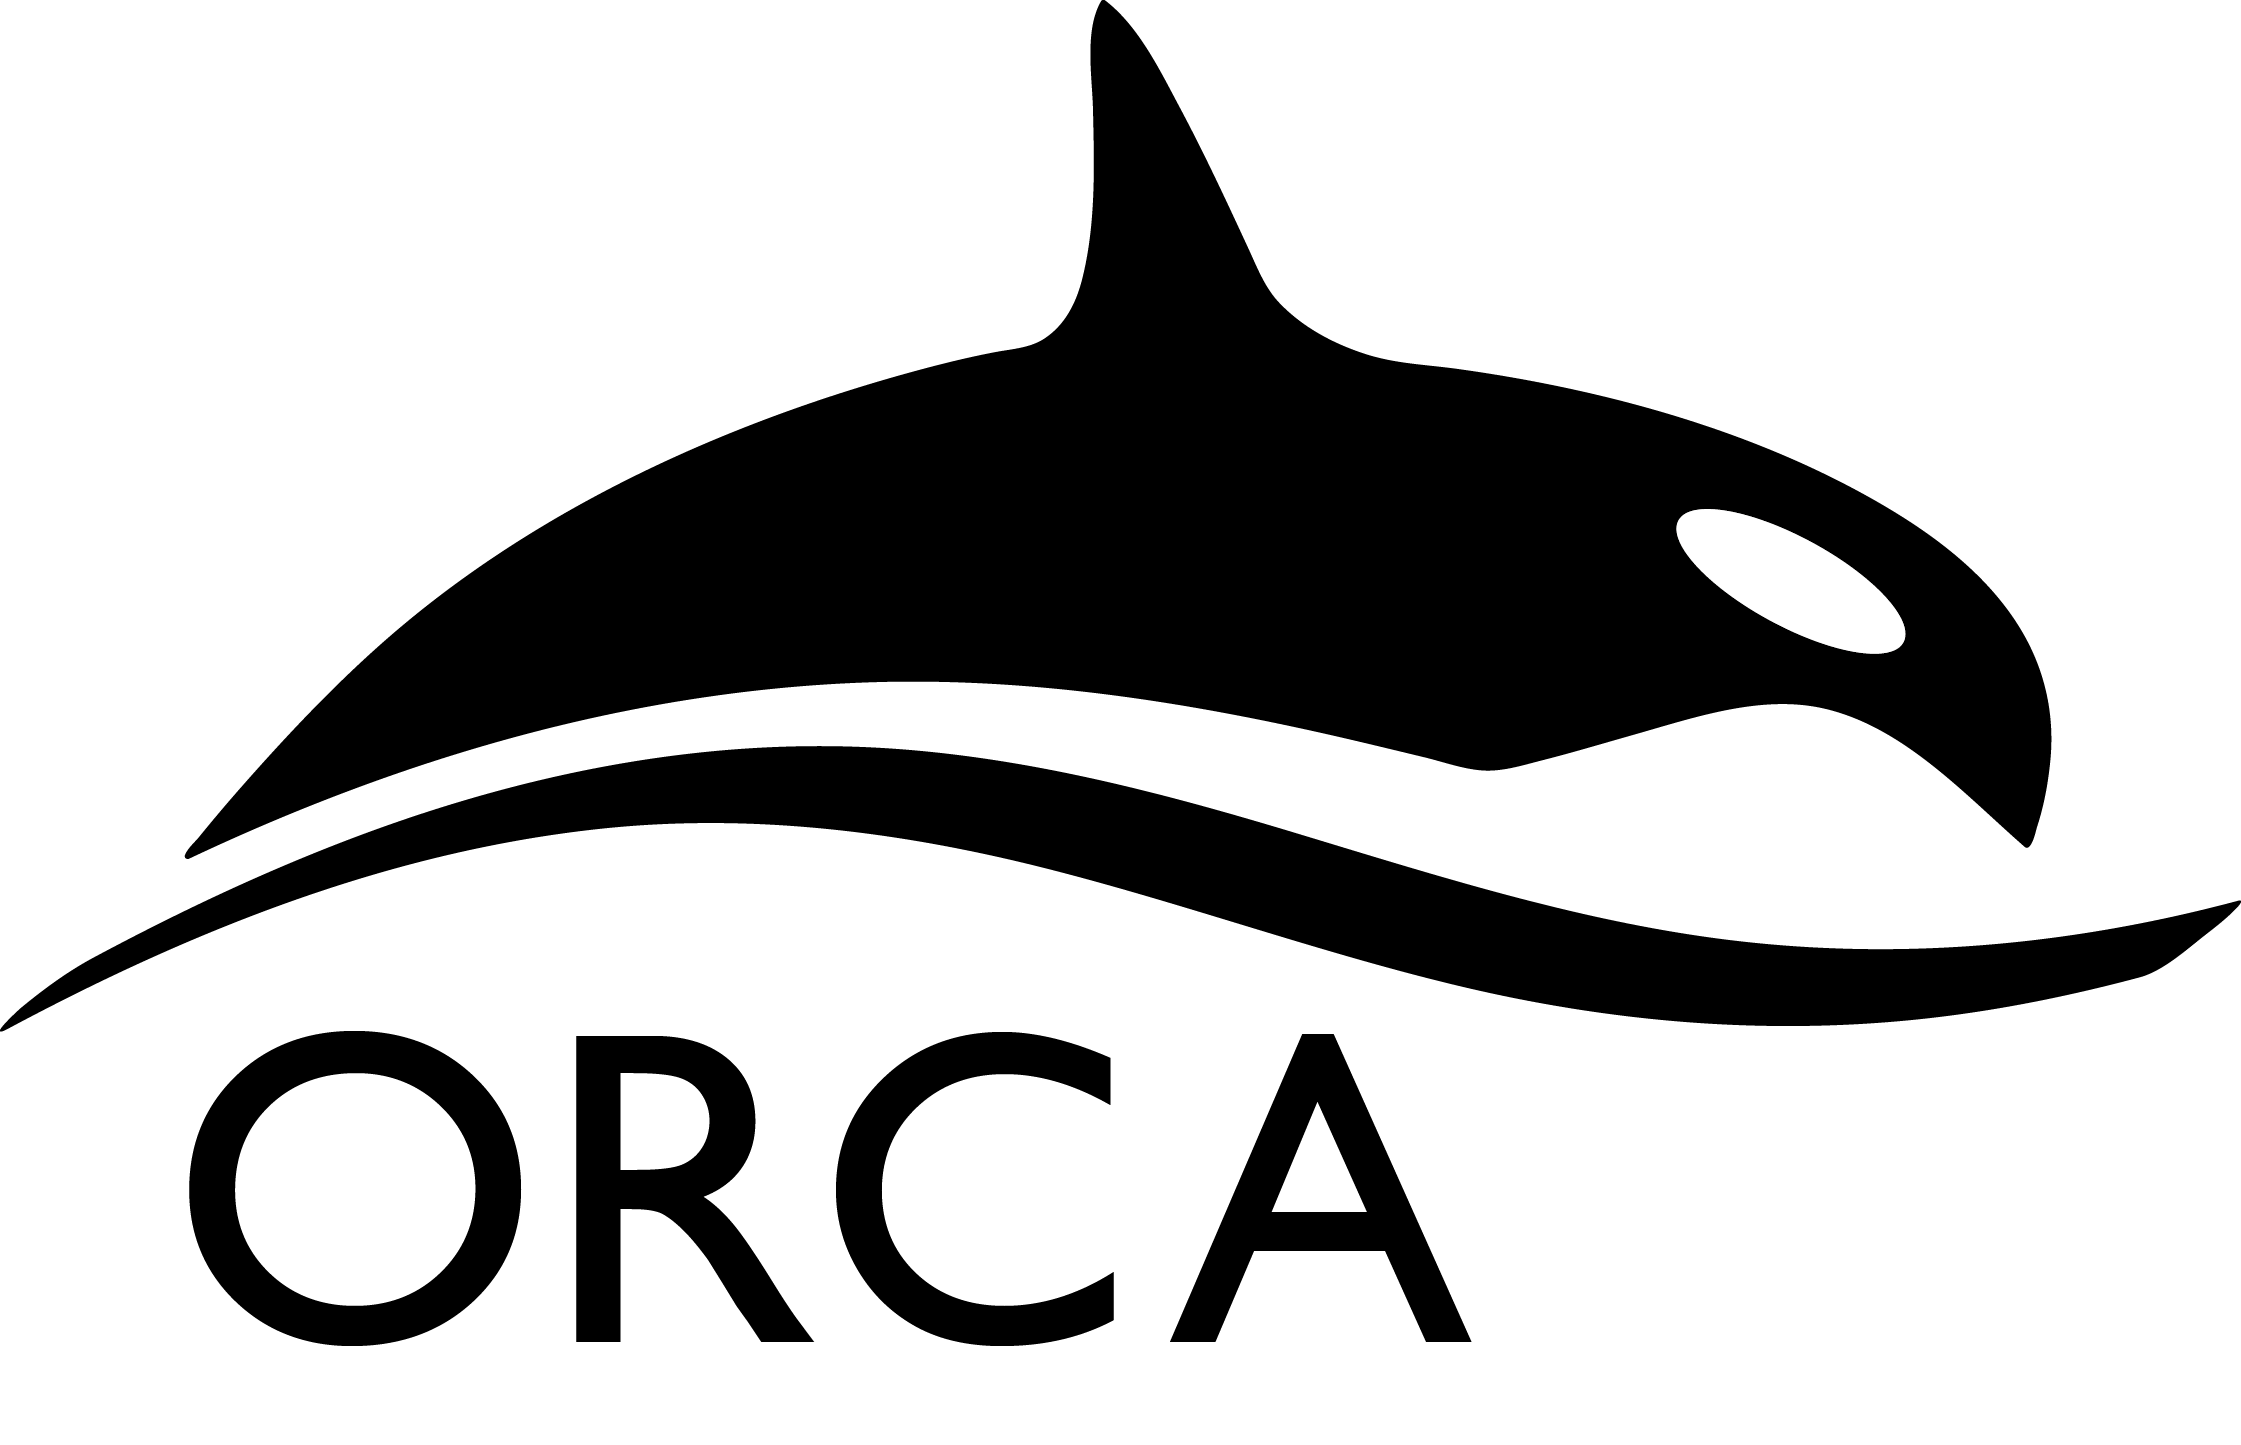
\includegraphics[width=180px]{/content/img/orca_logo_mpi.png}%
\caption{Logo del programa Orca}%
\end{figure}

%
Keywords: Organic Solar Cell, Small Molecules, Machine Learning, Computational Chemistry, Quantum Systems.

%
\end{document}